\documentclass[nojss]{jss}
\usepackage{booktabs,dcolumn,lmodern,amsmath}
\usepackage{Sweave}

\author{Simon Thielen\\Universit\"at Innsbruck}
\Plainauthor{Simon Thielen}

\title{Cumulative Booking Matrix for Historical Hotel Booking Data}

\Keywords{hotel, bookings, regression, \proglang{R}}
\Plainkeywords{hotel, bookings, regression, R}

\Abstract{
The \pkg{bookMatrix} package (\url{https://R-Forge.R-project.org/projects/uibk-rprog-2017/}) fits a cumulative booking matrix to analyze future hotel booking demand. A short overview of the package is provided and an exemplary regression analysis is done on an invented data set. Also descriptive statistics and illustrations are presented.
}

\Address{
  Simon Thielen\\
  Universit\"at Innsbruck\\
  Universit\"atsstr.~15\\
  6020 Innsbruck, Austria\\
  E-mail: \email{simon.thielen@student.uibk.ac.at}
}

%% Sweave/vignette information and metadata
%% need no \usepackage{Sweave}
%\VignetteIndexEntry{cumulative booking Matrix}
%\VignetteEngine{Sweave}




\begin{document}
\Sconcordance{concordance:bookMatrix-tex.tex:bookMatrix-tex.Rnw:%
1 29 1 1 5 22 1 1 2 1 0 2 1 4 0 1 2 11 1 1 2 1 0 1 2 1 0 1 1 4 0 1 2 7 %
1 1 4 20 1 1 12 3 1 1 2 41 0 1 2 6 1 1 2 9 0 1 1 9 0 1 2 8 1 1 2 1 0 4 %
1 1 4 3 0 1 1 1 4 3 0 1 1 1 4 7 0 1 2 6 1}


\section{Introduction}

Knowing the future demand of a hotel is important for hotel owners to improve their yield management strategies. The results of existing research show that there are many possibilities to fit an accurate forecasting model. The goodness of fit of these models depends on the needs of the user, time factors, location of the hotel and many other factors. In the following section accomplish a linear regression model that forecasts future booking demand. \\
To find valuable information through a first analysis by descriptive statistics the existing data can be edited in successive steps. Building a cumulative booking matrix of the initial data relieved the final regression process.


\section{Cumulative Booking Matrix}

The first step in the forecasting process is to edit the data so that all provided information on the bookings can be used in the analysis. The initial data frame includes a variable of the date of creation, the date of arrival and the date of departure. This data frame is transformed into a data frame that also provides the length of the customers stay (horizon).

\begin{verbatim}
findHorizon(hotelData, ...)
\end{verbatim}

The used data frame must contain the three main variables or it will be rejected.\\
To illustrate this in practice the packages functions are applied to a invented hotel booking data frame. The output do not contain any meaningful results.


\begin{Schunk}
\begin{Sinput}
> data("hoteldataRandom", package = "bookMatrix")
> hotelData <- findHorizon(hoteldataRandom)
> hist(hotelData$horizon, breaks = 100, main = "Figure 1: Horizon of the Bookings")
\end{Sinput}
\end{Schunk}
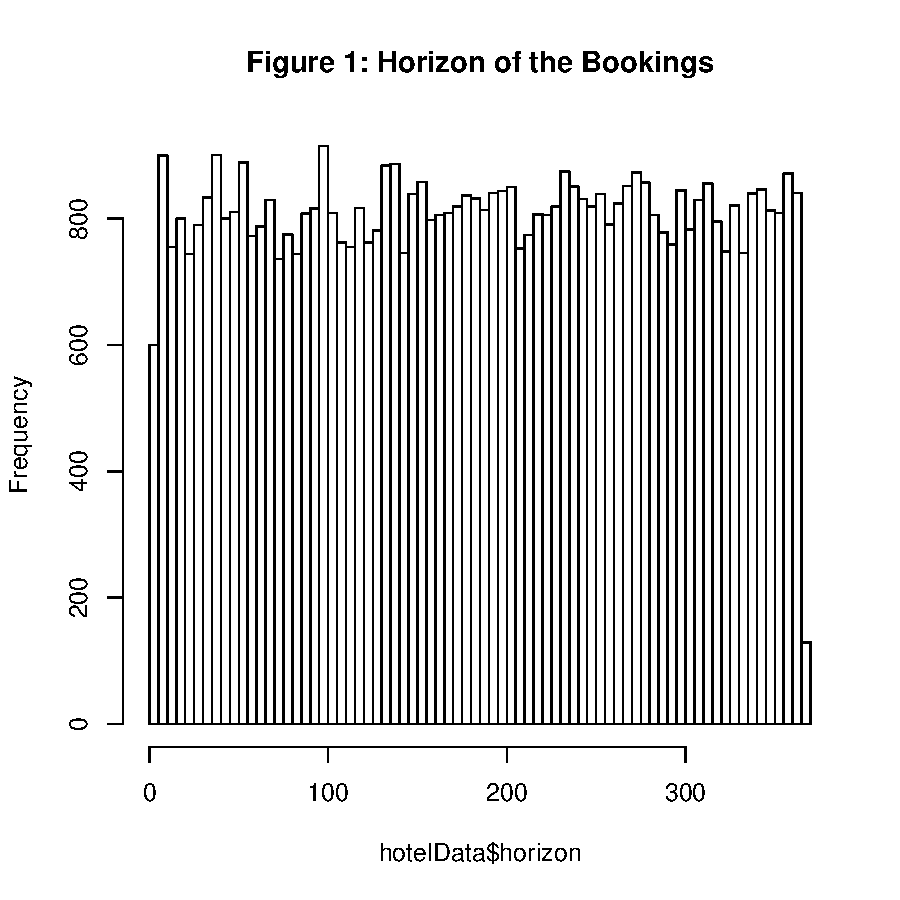
\includegraphics{bookMatrix-tex-002}


Looking at the invented example the distribution on the length of the stay seems approximately equally distributed. \\
The next step is converting this data frame into a cumulative booking matrix with the function fitCumuBookMat. 

\begin{verbatim}
fitCumuBookMat(hotelData, ...)
\end{verbatim}

This cumulative booking matrix stores the bookings as well as some information that can be used as controls in a future regression. These information might be time dependent factors, economic factors, characteristics of the customers or other pulling factors.
A target variable contains the final demand of bookings on a day. Different lag variables contain the amount of bookings for the day stored in the same row n days in the past. Here the number of the lag gives the information how many days the lag date back.

\begin{Schunk}
\begin{Sinput}
> cumBookMat <- fitCumuBookMat(hotelData=hotelData)
> plot(cumBookMat$date, cumBookMat$target, type="l", ylab="# Arrivals", 
+      xlab="Time", main = "Figure 2: Hotel Demand on Target Date")
> abline(h=mean(cumBookMat$target), col ="red")
\end{Sinput}
\end{Schunk}
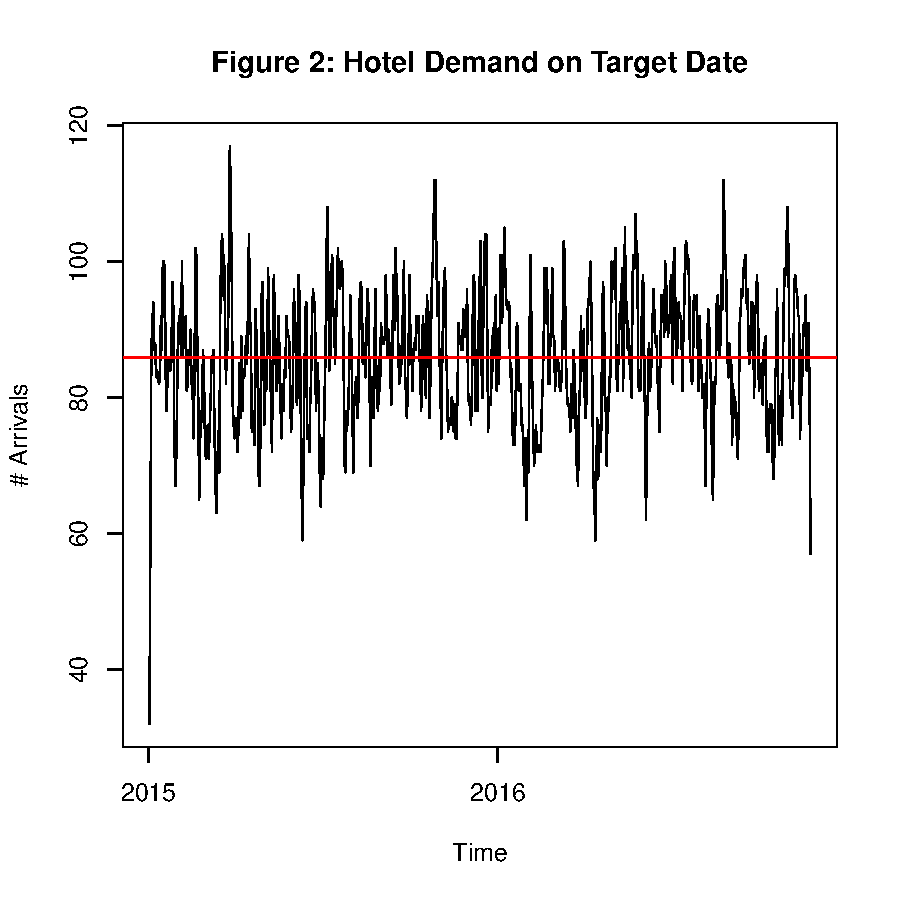
\includegraphics{bookMatrix-tex-003}

Figure 2 plots the time by days versus the arrivals on these days. The demand is distributed about the mean of approximately 86 over the given period.\\
In the next step it is possible to add a regressor that contains the amount of bookings exactly 365 lags before the regressor lag.

\begin{verbatim}
fitOneYearVar(cumBookMat, year1=2016, year2=2015, ...)
\end{verbatim}


Now the final design of the cumulative booking matrix is finished and can be used for further analysis.

\section{Linear Regression}

On this basis of this booking matrix regressions with various controls can be run and compared. The dependent variable is the logarithmic target variable with the final amount of bookings. The independent variables are one selected lag and the log of the same lag divided by the member lag that date back 365 lag. Different dummy controls can be added.

\begin{align*}
   log(target) = \beta_{0} + \beta_{1}*log(lag_{n}) + \beta_{2}*log(\frac{lag_{n}}{lag_{n,365}}) + \gamma*controls +         \epsilon
\end{align*}

The regression that fits the data best is than build over all provided lags. The goodness of fit is fitted to all these regressions and illustrated in a plot versus the lags.

\begin{verbatim}
runRegressions(data1, lag, year1=2016, year2=2015, 
                           oneyear=TRUE, wdayyes=TRUE, monthyes=TRUE, 
                           bayernholiday=TRUE,  publicholiday=TRUE,
                           italholiday=FALSE, season=FALSE, season2=FALSE, 
                           clear=FALSE, ...)
\end{verbatim}


With this function a regression can easily be computed and edited to the needs of the user. \\
It should contain all controls that the user might potentially connect to the amount of booking demand.

\begin{Schunk}
\begin{Sinput}
> mtable(linReg, linReg1, linReg2, summary.stats = c("R-squared", "sigma", "N") )
\end{Sinput}
\begin{Soutput}
Calls:
linReg: lm(formula = f, data = data1)
linReg1: lm(formula = f, data = data1)
linReg2: lm(formula = f, data = data1)

============================================================================
                                            linReg     linReg1    linReg2   
----------------------------------------------------------------------------
  (Intercept)                               0.806***   0.844***   0.845***  
                                           (0.107)    (0.104)    (0.104)    
  log(lag56 + 0.5)                          0.847***   0.839***   0.840***  
                                           (0.025)    (0.024)    (0.024)    
  I(log(lag56 + 0.5) - log(lagp56 + 0.5))   0.006      0.010      0.008     
                                           (0.017)    (0.017)    (0.017)    
  season: winterseason/noseason             0.012                           
                                           (0.006)                          
  season: summerseason/noseason             0.002                           
                                           (0.005)                          
  wday: Tue/Mon                                                   0.003     
                                                                 (0.009)    
  wday: Wen/Mon                                                  -0.005     
                                                                 (0.009)    
  wday: Thu/Mon                                                  -0.005     
                                                                 (0.009)    
  wday: Fri/Mon                                                  -0.013     
                                                                 (0.009)    
  wday: Sat/Mon                                                  -0.013     
                                                                 (0.009)    
  wday: Sun/Mon                                                  -0.007     
                                                                 (0.009)    
----------------------------------------------------------------------------
  R-squared                                    0.9        0.9        0.9    
  sigma                                        0.0        0.0        0.0    
  N                                          326        326        326      
============================================================================
\end{Soutput}
\end{Schunk}


\section{Model selection}

If the models are nested it is possible to just compare them by information criteria.
To consider the complexity of the model both AIC and BIC will be computed.

\begin{Schunk}
\begin{Sinput}
> AIC(linReg, linReg1, linReg2)
\end{Sinput}
\begin{Soutput}
        df       AIC
linReg   6 -1150.989
linReg1  4 -1151.448
linReg2 10 -1145.242
\end{Soutput}
\begin{Sinput}
> BIC(linReg, linReg1, linReg2)
\end{Sinput}
\begin{Soutput}
        df       BIC
linReg   6 -1128.267
linReg1  4 -1136.301
linReg2 10 -1107.373
\end{Soutput}
\end{Schunk}

If the fitting over all lags should be included in the model selection the R-squared over all lags can be computed and compared. The model that has on average the highest R-squared or in the section of interest should be used if the complexity of the model is not of interest.

\begin{verbatim}
rsq_by_lag(hotelData, r.squared=TRUE, ...)
\end{verbatim}

With this function the Rsquared over different periods can be build. It is also possible to find the coefficients of the first regressor over time if r.squared is FALSE.

\begin{Schunk}
\begin{Sinput}
> rsq0 <- rsq_by_lag(cumBookMat, oneyear = TRUE)
> rsq1 <- rsq_by_lag(cumBookMat, oneyear = TRUE, season = TRUE)
> rsq2 <- rsq_by_lag(cumBookMat, oneyear = TRUE, monthyes = TRUE)
> par(mfrow=c(1,3))
> plot(rsq ~ lag, data = rsq0, ylab = "R-squared", xlab = "Lag", type = "l", lwd = 2)
> legend("topright", "linReg",
+        lty = 1 , col = "black",
+        lwd = 2, bty = "n"
+ )
> plot(rsq ~ lag, data = rsq1, ylab = "R-squared", xlab = "Lag", type = "l", lwd = 2)
> legend("topright", "linReg1",
+        lty = 1 , col = "black",
+        lwd = 2, bty = "n"
+ )
> plot(rsq ~ lag, data = rsq2, ylab = "R-squared", xlab = "Lag", type = "l", lwd = 2)
> legend("topright", "linReg2",
+        lty = 1 , col = "black",
+        lwd = 2, bty = "n"
+ )
\end{Sinput}
\end{Schunk}
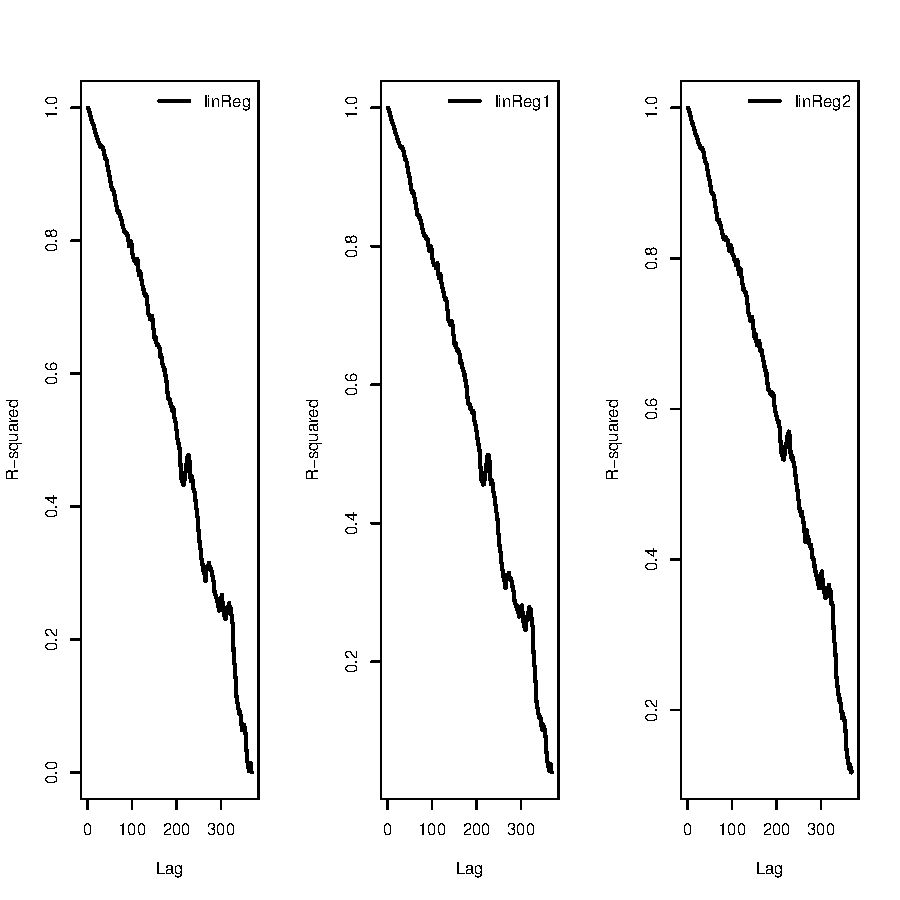
\includegraphics{bookMatrix-tex-008}

For the invented data there is not much difference between the R-squared over all lags between the three regressions. But previous tests with other data show a significant improve by including different controls. \\
While this is not given in this case it might be meaningful to take the model with the smallest information criteria. Therefore, model 3 (linReg2) is preferred to the other two regression models.


\end{document}

